% Numbers in this file are copied from tables/*.tex and reports/eval_review3/{summary,significance}.md.

\subsection{Implementation on Dataset 1: ACI-Bench}
Table~\ref{tab:aci} compares our systems with the published MEDIQA-Chat 2023 Task~B systems on ACI-Bench
test~1, scored with the official script. The untrained Llama-3.1-8B-Instruct (A) reaches ROUGE-1 0.519,
equal to the organisers' GPT-4 zero-shot baseline (0.518) and above ChatGPT (0.474), the fine-tuned LongT5
(0.431) and the GPT-3 system of GersteinLab (0.501). It stays below the best systems, which use GPT-4 with
retrieved in-context examples (0.614) or fine-tuned BART (0.530 with two-pass summarisation~\cite{sharma2023cadence};
0.535 when generating each note division separately~\cite{yim2023aci}). Adding the fact
table (B) leaves ROUGE essentially unchanged (0.516). The verifier (C) lowers ROUGE-1 to 0.462 because it
removes sentences. The QLoRA SFT model scores only 0.255: 89 of its 120 ACI-Bench notes reached the 1,024-token
limit and 70 were degenerate (repeated phrases or endless lists such as ``no history of nipple edema \ldots''),
because only 67 of its 4,265 training examples were full ACI-Bench notes. Giving it the fact table
(SFT + Fact table) does not help (0.208): the fine-tuned model ignores the added context and loops in the same way.
An earlier run with a 768-token limit scored 0.281; allowing more tokens only lengthened the loops, so the
low score is caused by degeneration, not by the length limit.

\begin{table}[t]
\centering
\caption{Dataset 1 --- ACI-Bench test 1 (40 full notes, MEDIQA-Chat 2023 Task B). ROUGE F1, official scoring. Published rows from~\cite{abacha2023overview}.}\label{tab:aci}
\scriptsize
\setlength{\tabcolsep}{2.5pt}
\resizebox{\columnwidth}{!}{\begin{tabular}{@{}llrrrr@{}}
\toprule
System & Method & R-1 & R-2 & R-L & R-Lsum\\
\midrule
WangLab~\cite{giorgi2023wanglab} & GPT-4 ICL & \textbf{0.614} & \textbf{0.329} & \textbf{0.382} & \textbf{0.551}\\
Cadence~\cite{sharma2023cadence} & BART FT & 0.530 & 0.250 & 0.298 & 0.466\\
iuteam1~\cite{abacha2023overview} & LSG-BART FT & 0.527 & 0.262 & 0.306 & 0.498\\
GersteinLab~\cite{abacha2023overview} & GPT-3 & 0.501 & 0.251 & 0.328 & 0.467\\
Calvados~\cite{abacha2023overview} & LongT5 FT & 0.431 & 0.202 & 0.239 & 0.386\\
Yim et al.~\cite{yim2023aci} & BART+SAMSum, by division & 0.535 & 0.251 & -- & --\\
Organisers~\cite{abacha2023overview} & GPT-4 0-shot & 0.518 & 0.226 & 0.303 & 0.426\\
Organisers~\cite{abacha2023overview} & ChatGPT 0-shot & 0.474 & 0.190 & 0.271 & 0.390\\\midrule
Ours: SFT (QLoRA) & Llama-3.1-8B & 0.255 & 0.101 & 0.159 & 0.231\\
Ours: SFT + Fact table & Llama-3.1-8B & 0.208 & 0.079 & 0.126 & 0.187\\
Ours: A. Zero-shot & Llama-3.1-8B & 0.519 & 0.214 & 0.297 & 0.477\\
Ours: B. + Fact table & Llama-3.1-8B & 0.516 & 0.214 & 0.295 & 0.474\\
Ours: C. + Verifier (FaCTS) & Llama-3.1-8B & 0.462 & 0.195 & 0.277 & 0.427\\
\bottomrule
\end{tabular}}
\end{table}


\subsection{Implementation on Dataset 2: MTS-Dialog}
On MTS-Dialog (Table~\ref{tab:mts}) the picture reverses. The SFT model reaches ROUGE-1 0.400 on test~1,
level with GersteinLab (0.401) and Calvados (0.395) and above both organiser baselines (GPT-4 0.307,
ChatGPT 0.303); on all 400 test items it reaches 0.392, above the prompt-tuned GatorTronGPT-20B (0.363) and
the fully fine-tuned T5-Large (0.343) of~\cite{lyu2024}. The zero-shot model scores 0.303, the same as GPT-4
zero-shot. With the fact table the SFT model scores 0.382 (test~1) and 0.372 (all 400).
MTS-Dialog references are very short (median 14 words); fine-tuning teaches the model this
terse style, whereas the base model writes full sentences (``The patient presents with a complaint of a
boil-like condition located on their buttocks'' for the reference ``Buttock abscess.''), which lowers lexical
overlap without being wrong. Our prompt contains the gold section header, whereas Task~A teams also had to
predict it.

\begin{table}[t]
\centering
\caption{Dataset 2 --- MTS-Dialog. Top: test 1 (200, MEDIQA-Chat 2023 Task A~\cite{abacha2023overview}). Bottom: both test sets (400) vs.~\cite{lyu2024}. ROUGE F1, official scoring.}\label{tab:mts}
\scriptsize
\setlength{\tabcolsep}{2.5pt}
\resizebox{\columnwidth}{!}{\begin{tabular}{@{}llrrr@{}}
\toprule
System & Method & R-1 & R-2 & R-L\\
\midrule
\multicolumn{5}{@{}l}{\emph{Test 1 (200)}}\\
WangLab~\cite{giorgi2023wanglab} & GPT-4 ICL & \textbf{0.447} & \textbf{0.228} & \textbf{0.384}\\
Cadence~\cite{sharma2023cadence} & BART FT & 0.430 & 0.208 & 0.364\\
GersteinLab~\cite{abacha2023overview} & FT + ICL & 0.401 & 0.215 & 0.332\\
Calvados~\cite{abacha2023overview} & LongT5 FT & 0.395 & 0.186 & 0.332\\
Care4Lang~\cite{abacha2023overview} & LM FT & 0.358 & 0.165 & 0.289\\
Organisers~\cite{abacha2023overview} & GPT-4 0-shot & 0.307 & 0.128 & 0.236\\
Organisers~\cite{abacha2023overview} & ChatGPT 0-shot & 0.303 & 0.121 & 0.242\\\midrule
Ours: SFT (QLoRA) & Llama-3.1-8B & 0.400 & 0.183 & 0.342\\
Ours: SFT + Fact table & Llama-3.1-8B & 0.382 & 0.175 & 0.326\\
Ours: A. Zero-shot & Llama-3.1-8B & 0.303 & 0.106 & 0.235\\
Ours: B. + Fact table & Llama-3.1-8B & 0.294 & 0.117 & 0.227\\
Ours: C. + Verifier (FaCTS) & Llama-3.1-8B & 0.287 & 0.114 & 0.225\\
\midrule
\multicolumn{5}{@{}l}{\emph{Test 1 + 2 (400)}}\\
Lyu et al.~\cite{lyu2024} & GatorTronGPT-20B PT & 0.363 & 0.155 & \textbf{0.347}\\
Lyu et al.~\cite{lyu2024} & T5-Large FT & 0.343 & 0.146 & 0.337\\\midrule
Ours: SFT (QLoRA) & Llama-3.1-8B & \textbf{0.392} & \textbf{0.168} & 0.333\\
Ours: SFT + Fact table & Llama-3.1-8B & 0.371 & 0.164 & 0.313\\
Ours: A. Zero-shot & Llama-3.1-8B & 0.310 & 0.108 & 0.240\\
Ours: B. + Fact table & Llama-3.1-8B & 0.285 & 0.106 & 0.215\\
Ours: C. + Verifier (FaCTS) & Llama-3.1-8B & 0.275 & 0.102 & 0.213\\
\bottomrule
\end{tabular}}
\end{table}


\subsection{Clinical factuality on both datasets}
Table~\ref{tab:fact} reports the factuality metrics on all test items and Fig.~\ref{fig:fact} summarises
them; Table~\ref{tab:sig} gives paired differences with bootstrap confidence intervals.

\emph{Fine-tuning increases hallucination.} With the same prompt, the SFT model hallucinates 51.7\% of its
clinical entities on ACI-Bench and 35.6\% on MTS-Dialog, against 14.4\% and 20.4\% for the untrained model
(paired differences $+37.3$ and $+14.3$ points, both significant). On ACI-Bench it also flips more
negations ($+9.0$), invents more numbers (numerical consistency $-26.2$) and covers fewer reference facts
($-29.6$). On MTS-Dialog, where only 12 of 400 SFT notes were truncated, the hallucination increase remains
significant while ROUGE-L \emph{improves} by 9.5 points: the model learned the form of the notes faster
than their grounding. This agrees with the general-domain finding that fine-tuning on unknown facts
increases hallucination~\cite{gekhman2024} and with the doubled hallucination count reported for SFT of the
same base model on discharge notes~\cite{seethakantha2026hdsr}.
Adding the fact table to the SFT model lowers its hallucination on MTS-Dialog (35.6\%$\rightarrow$28.3\%,
$-4.3$ paired, significant) but not on ACI-Bench (51.2\%, $-0.6$, not significant), and it increases negation
flips on both datasets ($+4.0$ and $+3.0$). Even with the fact table the SFT model hallucinates about twice as
often as the untrained model with the same prompt (B), so the fact table cannot repair what fine-tuning broke.

\emph{The fact table reduces hallucination without losing coverage.} Conditioning on the extracted facts
(B) lowers hallucination by 3.9 points on ACI-Bench (14.4\%$\rightarrow$10.6\%) and by 3.5 points on
MTS-Dialog (paired; 20.4\%$\rightarrow$15.8\% over all items), both significant, and raises numerical
consistency on ACI-Bench from 83.7\% to 93.0\%, because doses and measurements are listed explicitly.
Coverage does not drop (77.2\% vs.\ 76.8\% on ACI-Bench; 71.5\% vs.\ 68.0\% on MTS-Dialog), so B has the best
fact-level F1 on both datasets (82.8 and 77.4). Negation flips do not change significantly.

\emph{Drop-only verification trades coverage for precision.} The verifier (C) gives the lowest
hallucination rate on both datasets (8.7\% and 14.2\%), but the reduction over B is small (significant only on
ACI-Bench, $-1.8$ points) while coverage falls by 11.6 and 10.6 points. Removing a sentence that contains one
unsupported entity also removes the supported facts in it. FaCTS with the verifier is therefore a
high-precision mode; the fact-conditioned generator alone gives the best balance.

\begin{table*}[t]
\centering
\caption{Clinical factuality on all test items of each dataset (per-item means, \%). R-L uses stemming; BERTScore = roberta-large, rescaled. Halluc.\ and Neg.\ flip: lower is better. $P_f=1-$Halluc., $R_f=$ Coverage.}\label{tab:fact}
\footnotesize
\resizebox{\textwidth}{!}{\begin{tabular}{@{}lrrrrrrrrr@{}}
\toprule
System & R-L & BERTScore & Halluc.$\downarrow$ & Neg.\ flip$\downarrow$ & Num.\ cons. & Coverage & $P_f$ & $R_f$ & $F1_f$\\
\midrule
\multicolumn{10}{@{}l}{\emph{ACI-Bench (120)}}\\
SFT (QLoRA) & 16.4 & -0.022 & 51.7 & 13.7 & 57.6 & 47.2 & 48.3 & 47.2 & 47.7\\
SFT + Fact table & 13.3 & -0.102 & 51.2 & 17.7 & 62.6 & 50.7 & 48.8 & 50.7 & 49.7\\
A. Zero-shot & 30.4 & 0.224 & 14.4 & 4.7 & 83.7 & 76.8 & 85.6 & 76.8 & 80.9\\
B. + Fact table & 29.7 & 0.219 & 10.6 & 4.7 & 93.0 & 77.2 & 89.4 & 77.2 & 82.8\\
C. + Verifier (FaCTS) & 27.8 & 0.181 & 8.7 & 3.8 & 93.6 & 65.6 & 91.3 & 65.6 & 76.3\\
\midrule
\multicolumn{10}{@{}l}{\emph{MTS-Dialog (400)}}\\
SFT (QLoRA) & 34.6 & 0.428 & 35.6 & 5.1 & 82.9 & 68.1 & 64.4 & 68.1 & 66.2\\
SFT + Fact table & 32.4 & 0.411 & 28.3 & 8.4 & 80.7 & 69.8 & 71.7 & 69.8 & 70.8\\
A. Zero-shot & 25.1 & 0.223 & 20.4 & 4.9 & 88.3 & 68.0 & 79.6 & 68.0 & 73.3\\
B. + Fact table & 22.4 & 0.224 & 15.8 & 5.4 & 84.4 & 71.5 & 84.2 & 71.5 & 77.4\\
C. + Verifier (FaCTS) & 22.3 & 0.212 & 14.2 & 6.2 & 85.1 & 60.9 & 85.8 & 60.9 & 71.3\\
\bottomrule
\end{tabular}}
\end{table*}


\begin{figure}[t]
\centering
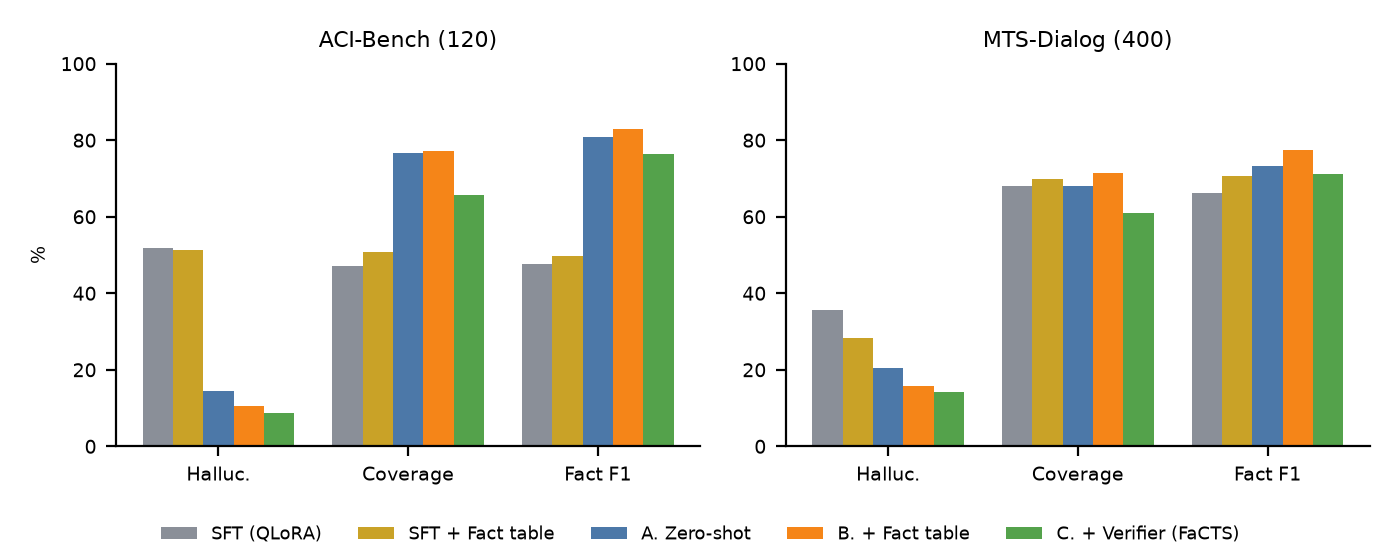
\includegraphics[width=\columnwidth]{figures/factuality.png}
\caption{Hallucination rate, coverage and fact-level F1 per system and dataset (all test items).}\label{fig:fact}
\end{figure}

\begin{table}[t]
\centering
\caption{Paired differences in percentage points (per-item means). $^{*}$: 95\% paired bootstrap interval excludes 0 (10{,}000 resamples).}\label{tab:sig}
\scriptsize
\setlength{\tabcolsep}{2.5pt}
\resizebox{\columnwidth}{!}{\begin{tabular}{@{}llrrrrr@{}}
\toprule
Dataset & Comparison & Halluc. & Neg.\ flip & Num.\ cons. & Coverage & R-L\\
\midrule
ACI-Bench & SFT $-$ A & +37.3$^{*}$ & +9.0$^{*}$ & -26.2$^{*}$ & -29.6$^{*}$ & -14.0$^{*}$\\
ACI-Bench & SFT+F $-$ SFT & -0.6 & +4.0$^{*}$ & +5.5 & +3.5 & -3.1$^{*}$\\
ACI-Bench & B $-$ A & -3.9$^{*}$ & -0.0 & +9.4$^{*}$ & +0.4 & -0.7$^{*}$\\
ACI-Bench & C $-$ B & -1.8$^{*}$ & -0.8 & +0.8 & -11.6$^{*}$ & -1.8$^{*}$\\
\midrule
MTS-Dialog & SFT $-$ A & +14.3$^{*}$ & +1.2 & -5.4$^{*}$ & +0.1 & +9.5$^{*}$\\
MTS-Dialog & SFT+F $-$ SFT & -4.3$^{*}$ & +3.0$^{*}$ & -1.6 & +1.7 & -2.1$^{*}$\\
MTS-Dialog & B $-$ A & -3.5$^{*}$ & +1.2 & -0.7 & +3.6 & -2.7$^{*}$\\
MTS-Dialog & C $-$ B & -0.7 & +0.3 & +2.3$^{*}$ & -10.6$^{*}$ & -0.1\\
\bottomrule
\end{tabular}}
\end{table}


\subsection{Verifier analysis}\label{sec:ver}
The evidence strategy of the verifier was chosen on the validation sets only. Reference sentences of the
120 ACI-Bench and MTS-Dialog validation notes should pass; copies with one injected negation flip or changed
number should fail. With the selected strategy (maximum over whole transcript, top-3 windows and their
union), the verifier passed 72.8\% of 966 reference sentences and caught 60.6\% of 302 corrupted ones (75.4\%
of number changes but only 35.1\% of negation flips), a balanced accuracy of 0.667, against 0.648 for
a single retrieved premise and 0.639 with five windows. Because human references contain some content that
was never said, the pass rate is a lower bound. On the test notes of system B the verifier marked 28.8\% of the
checked sentences red on both datasets (Table~\ref{tab:ver}); no note was emptied. Its weakness on negation
mirrors the finding that general-domain detectors struggle on clinical dialogue~\cite{bn2025fact}.

\begin{table}[t]
\centering
\caption{Verifier verdicts on system B notes (share of checked sentences, \%). Red sentences are dropped.}\label{tab:ver}
\scriptsize
\setlength{\tabcolsep}{3pt}
\resizebox{\columnwidth}{!}{\begin{tabular}{@{}lrrrrrr@{}}
\toprule
Dataset & Notes & Sent. & Green & Yellow & Red & Emptied\\
\midrule
ACI-Bench (120) & 120 & 2905 & 68.0 & 3.2 & 28.8 & 0\\
MTS-Dialog (400) & 400 & 1506 & 69.5 & 1.7 & 28.8 & 0\\
\bottomrule
\end{tabular}}
\end{table}


\subsection{Discussion and limitations}
Three results hold on both datasets with significant paired differences: QLoRA fine-tuning raised
hallucination, the fact table lowered it, and the verifier lowered coverage. Lexical metrics alone would
have ranked the SFT model best on MTS-Dialog, which is why factuality metrics must be reported next to
ROUGE.

The study has limitations. (1) Factuality is measured automatically with our lexicon-based extractor;
human reference notes themselves score 15\% (ACI-Bench) and 28\% (MTS-Dialog) ``hallucination'' under this
metric, which is therefore a floor, not zero, and no clinician evaluation was performed. (2) The SFT
adapter was selected by validation loss on data with few full ACI-Bench notes; a rebalanced adapter might
degenerate less, so its ACI-Bench numbers describe this adapter, not SFT in general. (3) BLEURT and the
deberta-xlarge BERTScore of the shared task were not computed, so only ROUGE is compared with published
systems. (4) MTS-Dialog prompts include the gold section header. (5) All results are from one greedy run.
